
%-----------------------------------------------------------------------------
% Chapter: Development
%-----------------------------------------------------------------------------

\chapter{Development}
\label{chap:DEV}

\section{Methodology}
The most important point in the development process of the \emph{Course2018}
LMS is the idea of \emph{continuous integration} (CI), meaning that every new
develop feature is tested and integrated to the existing server seamlessly.

\medskip
This is achieved by using a development tool called \emph{GitLab CI}
\cite{gitlabCI}, a sub-system that came with the source management tool,
\emph{GitLab}~\cite{gitlab}, which is also used for the development of this
project. 

\medskip

This toolchain offers abilities to a developer so that every time
the developer finishes programming of a feature and pushes the code to the
\emph{GitLab} project repository, the \emph{GitLab} server automatically
invokes some
routines to test the new code with a test scheme also defined by the developer
prior to the time when the code was pushed; if all tests are passed, 
the \emph{GitLab} server then deploys the new version of the project by simply
building a new container that has the latest code in it, and has the old
container replaced with the new one. 

\section{Deployment}
In the development process of this project, the deployment stage is defined
before the actual programming even start. This approach makes sure that all
modules of the project can be test in the
deployment environment (i.e., the container in which the \emph{Course2018}
will be eventually running) as soon as the implementation if finished.

\subsection{Environment}
The \emph{Course2018} LMS is containerized in an environment
(the production container) based on
\emph{Debian 8}~\cite{debian}, with \emph{Python 3} and all necessary packages
(including \emph{Django 2.0}) installed.

\subsection{HTTP server}
An \emph{HTTP server} is included in the production container to host the
\emph{Course2018} LMS.
The \emph{HTTP server} in use in the production container is the
\emph{Apache HTTP server} (version 2.4)~\cite{apache}, with the
\texttt{mod\_wsgi}~\cite{wsgi} package installed to accommodate
\emph{Python} web applications in \emph{WSGI}
(Web Server Gateway Interface~\cite{wsgi}) specification, such as a
\emph{Django} project.

\section{System development}

\subsection{MVT}
\label{sec:MVT}
The \emph{Django} framework enforces developers to apply an architectural
pattern called the \emph{MVT} (Model-View-Template) pattern to their projects.
In such projects,
all data models are defined as \texttt{Model} classes, which
then are used to create schemas for corresponding database tables;
the data in the data models will then be retrieved and organized in 
methods of different \texttt{View} classes, each of these \texttt{View} classes
is connected to a \emph{URL};
webpages will finally be generated by those \texttt{View} classes
using different \emph{HTML} \texttt{Templates} with the organized data.

\subsection{APIs}
In the \emph{Course2018} LMS, some views are not paired with templates, and
they do not return webpages to the users, instead, they return some
\emph{JSON}-formatted data.
These views are the APIs (application programming interface) of the system,
and they are used for updating information in
a loaded page dynamically with \emph{AJAX}~\cite{AJAX}. 


%-----------------------------------------------------------------------------
% Section: User authentication
%-----------------------------------------------------------------------------

\subsection{User authentication}
As discussed in section~\ref{sec:USRAUTH}, user authentication is handled by the
\emph{Django User Model} provided by the \emph{Django} \texttt{auth} library,
not only does this approach simplifies the implementation of the module,
security is also improved in comparison with implementing the authentication
module solely by the developer.

\subsubsection{Data model}
Data model of the user authentication module is shown in
Figure~\ref{fig:AUTH_ER}, Table~\ref{tab:USR_ATTR} and
Table~\ref{tab:PROFILE_ATTR}.

\bigskip

\begin{figure}[ht]
    \centering
    \caption{Data model of the user authentication module}
    \usetikzlibrary{er}
    \label{fig:AUTH_ER}

    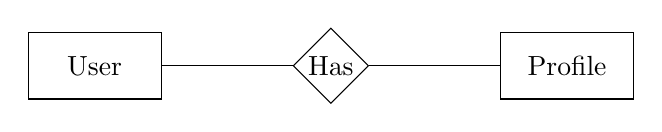
\begin{tikzpicture}[node distance = 3cm]
        \node[entity] (user) {User};
        \node[relationship] (has) [right of=user] {Has} edge (user);
        \node[entity] (profile) [right of=has] {Profile} edge (has);
    \end{tikzpicture}
\end{figure}


\begin{table}[ht]
    \centering
    \caption{Attributes of \texttt{User} model}
    \label{tab:USR_ATTR}
    \renewcommand{\arraystretch}{1.5}
    \begin{tabular}[ht]{r|l}
        \hline
        \texttt{Attribute} & Note \\
        \hline
        \hline
        \texttt{id} & primary key \\
        \hline
        \texttt{username} &  required, max length: 150 \\
        \hline
        \texttt{first\_name} &  optional, max length: 30 \\
        \hline
        \texttt{last\_name} &  optional, max length: 150 \\
        \hline
        \texttt{email} & optional\\
        \hline
        \texttt{password} & A hash of the user's password \\
        \hline
        \texttt{is\_active} & \texttt{boolean field}, indicating whether or not the user
            is active \\
        \hline
        \texttt{last\_lgoin} & \texttt{datetime field}, last login time \\
        \hline
        \texttt{data\_joined} & \texttt{datetime field}, time when the account is created \\
        \hline
    \end{tabular}
    \renewcommand{\arraystretch}{1}
\end{table}

\begin{table}[ht]
    \centering
    \caption{Attributes of \texttt{Profile} model}
    \label{tab:PROFILE_ATTR}
    \renewcommand{\arraystretch}{1.5}
    \begin{tabular}[ht]{r|l}
        \hline
        Attribute & Note \\
        \hline
        \hline
        \texttt{user\_id} & foreign key to a \texttt{User} model instance \\
        \hline
        \texttt{role} & \texttt{integer field}, choice from 0 and 1, indicating the
            user's role \\
           & is \emph{Student} or \emph{Professor} respectively \\
        \hline
    \end{tabular}
    \renewcommand{\arraystretch}{1}
\end{table}


\subsubsection{Views}

\begin{itemize}
    \item Login: \\
        A \texttt{UserLogin} view is defined to provide routines to handle user
        authentications, by invoking the built-in \emph{Django} library
        function~\texttt{authenticate()}
        to compare the credentials provided
        by the user against the user account database.

    \item Permission control: \\
        An abstract view class called \texttt{AbstractLoginRequiredView} is
        defined for general permission control. This class contains a function
        to check whether or not a user is authenticated, if the user is
        authenticated, the function then checks the role of the user and
        invokes \texttt{student\_view()} or \texttt{professor\_view()} to
        provide different content according to the user's role.

        All the views of the modules that require permission control are
        inherited from the \texttt{AbstractLoginRequiredView} class, and have
        the class function \\ \texttt{student\_view()} and
        \texttt{professor\_vew()} overridden to provide module-specific
        content for students and instructors respectively.

        In addition to that, there is also another abstract view class, \\
        \texttt{AbstractLoginRequiredAPI}, this class provides permission
        control for all the APIs in the same manner as discussed above.
\end{itemize}

\subsubsection{Templates}

\begin{itemize}
    \item Login template: \\
        This template is used by the \texttt{UserLogin} view to provide a very
        simple login interface to the users, it contains a form with two
        fields (username and password) and a \emph{Login} button. User can
        use this interface to log into the \emph{Course2018} LMS.
\end{itemize}


%-----------------------------------------------------------------------------
% Section: Course management
%-----------------------------------------------------------------------------

\subsection{Course management}
To provide source code management for programming assignments,
a great open-source version control tool,
\emph{Git}, is integrated to the \emph{Course2018} LMS,
this was originally developed by \emph{Linus Torvalds}~\cite{git},
creator and principal developer of the \emph{Linux} operating system
kernel~\cite{lTorvalds}.
Moreover, 
an open-source Git-repository manager, \emph{GitLab}~\cite{gitlab}, is also
used in the \emph{Course2018} LMS to enhance the source code management user
experience.

\medskip
Once an instructor enables source code management for an assignment, a remote
\emph{GitLab} repository is also created for the course to which the assignment
belongs. The name of the repository will be saved in the course management
module.

\medskip
Note that course materials feature is planned but not implemented due to the
limit of development time frame (see section {\bf TODO: REF FUTURE WORK}).

\subsubsection{Data model}
Data model of the user authentication module is shown in
Figure~\ref{fig:COURSE_ER} and Table~\ref{tab:COURSE_ATTR}. \bigskip

\begin{figure}[ht]
    \centering
    \caption{Data model of the course management module}
    \label{fig:COURSE_ER}
    \usetikzlibrary{er}

    \begin{tikzpicture}[scale=0.8, every node/.style={scale=0.8}, node distance = 4cm]
        \node[entity] (course) {Course};

        \node[relationship] (stu_reg) [below of=course] {Student} edge[total] (course);
        \node[entity] (stu) [left of = stu_reg] {User (Role: student)} edge[total] (stu_reg);

        \node[relationship] (instructor) [above of = course] {Instructor} edge (course);
        \node[entity] (prof) [left of = instructor] {User (Role: professor)} edge (instructor);

        \node[relationship] (ta_reg) [right of = course] {TA} edge[total] (course);
        \node[entity] (ta) [right of = ta_reg] {User} edge[total] (ta_reg);
    \end{tikzpicture}
\end{figure}

\begin{table}[ht]
    \centering
    \caption{Attributes of \texttt{Course} model}
    \label{tab:COURSE_ATTR}
    \renewcommand{\arraystretch}{1.5}
    \begin{tabular}[ht]{r|l}
        \hline
        \texttt{Attribute} & Note \\
        \hline
        \hline
        \texttt{id} & primary key \\
        \hline
        \texttt{department} & required, department code of the course \\ & (e.g., COMP, MATH) \\
        \hline
        \texttt{number} & required, course number \\
        \hline
        \texttt{section} & required, course section (e.g., X1) \\
        \hline
        \texttt{title} & require, course title \\
        \hline
        \texttt{semester} & required, semester of the course (e.g., Winter, Fall) \\
        \hline
        \texttt{start\_time} & required, \texttt{date} field, date the course
            becomes available to \\ & students \\
        \hline
        \texttt{end\_time} & required, \texttt{date} field, date the course ends \\
        \hline
        \texttt{visible\_after\_end} & required, \texttt{boolean} field, indicating
            whether or not to allow\\ & students access the course after it ends \\

        \hline
        \hline

        \texttt{instructor} & foreign key to the instructor \\
        \hline
        \texttt{students} & many to many relationship to the students registered \\ & in the course\\
        \hline
        \texttt{TAs} & many to many relationship to the TAs registered \\ & in the course \\

        \hline
        \hline

        \texttt{repo\_name} & optional, the name of the remote \emph{GitLab}
            repository \\ & in 
            which programming assignment source code files \\ & are stored \\
        \hline
        \hline

        \texttt{constraints} & 
            1. combination of fields
                \texttt{department},
                \texttt{number},
                \texttt{section}, \\ &
                \hspace{1.3em}\texttt{year},
                \texttt{semester} must be unique \\
            & 2. role of the \texttt{instructor} must be \emph{Professor} \\
            & 3. role of the each of the \texttt{students} must be \emph{Student} \\
        \hline
    \end{tabular}
    \renewcommand{\arraystretch}{1}
    
\end{table}

\subsubsection{Views}

\begin{itemize}
    \item Create courses: \\
        This activity is handled with the \texttt{CreateCourseView} which is
        inherited from the \texttt{AbstractLoginRequiredView} and 
        only accessible by instructors. 
        This view accepts all the \emph{create course} request, validates the
        data in the request, and if the data has no error,
        create a course record with the data.
        The permission control of this view
        (and any other views that are only accessible by instructors) is
        achieved by simply raising an \texttt{HTTPForbidden}~\cite{http403}
        error in the overridden \texttt{student\_view()} class function.
    
    \item View course summary:\\
    When a user send a \emph{view course} request to the server, the request
    is handled with a \texttt{CourseSummaryView} class which is inherited from
    the \texttt{AbstractLoginRequir-\\edView} class.
    \begin{itemize}
        \item \texttt{student\_view()}: 
            Information about the course and a list of assignments
            are fetched from the database and displayed to the registered
            students.
        \item \texttt{professor\_view()}: In addition to the course information,
            this function also fetches the latest students and TAs activities 
            (i.e., assignment submit activities and  assignment grading
            activities),
            and calculates the latest assignment's proportion of the student
            grades.
    \end{itemize}
\end{itemize}

\subsubsection{Templates}
\begin{itemize}
    \item Create course template: \\
        This template is used by the \texttt{CreateCourseView}, the template
        contains a form to be filled out by the user who
        wishes to create a course. 
    \item Course summary template:
    \begin{itemize}
        \item Student template: a web page with the course information
            (e.g., department, number, section, and title)
            displayed as the page title, and a list of assignments displayed
            in a table.
        \item Professor template: same page title displayed with the course
            information as in the student template;
            page content are divided into three sections:
            \begin{enumerate}
                \item Manage area where an instructor can add and remove
                    students, TAs, and assignments.
                \item Latest assignment statistics area where the latest
                    assignment's student grades proportion is displayed
                    in a horizontal bar chart.
                \item Latest activities area where the latest TA and student
                    activities are displayed in tables.
            \end{enumerate}
    \end{itemize}
\end{itemize}




%-----------------------------------------------------------------------------
% Section: Assignment management
%-----------------------------------------------------------------------------

\section{Assignment management}

\subsection{Data model}
Data model of the user authentication module is shown in
% Figure~\ref{fig:COURSE_ER} and Table~\ref{tab:COURSE_ATTR}. \bigskip

\begin{figure}[ht]
    \centering
    \caption{Data model of the assignment management module}
    \label{fig:ASM_ER}
    \usetikzlibrary{er}

    \begin{tikzpicture}[scale=0.8, every node/.style={scale=0.8}, node distance = 4cm]
        \node[entity] (course) {Course};

        \node[relationship] (course_asm) [below of =course] {has} edge (course);
        \node[entity] (asm) [below of = course_asm] {Assignment} edge[total] (course_asm);

        \node[relationship] (asm_commit) [below of = asm] {has} edge (asm);
        \node[entity] (commit) [below of = asm_commit] {Commit} edge[total] (asm_commit);

        \node[relationship] (ta_grade) [right of = commit] {grades} edge[total] (commit);
        \node[entity] (ta) [right of = asm] {User (TA)} edge (ta_grade) edge (ta_grade);

        \node[relationship] (commit_stu) [left of = commit] {creates} edge (commit);
        \node[entity] (stu) [left of = asm] {User (Student)} edge (commit_stu);

    \end{tikzpicture}
\end{figure}